\documentclass{article} 

\usepackage[utf8]{inputenc}
\usepackage{graphicx}
\usepackage[hidelinks]{hyperref} 

\renewcommand{\baselinestretch}{1.5}

\title{\Huge ADOO.\vspace{1 cm}  \\ Modelo en espiral \vspace{1 cm} }


\author{\\ \Huge Arturo Escutia López.\vspace{2 cm}\\ \Huge Profesor:Ulises Velez Saldaña}
\date{\Huge\vspace{2 cm}Septiembre 22 , 2015 \Huge  \vspace{2 cm} \\2CM12 \vspace{4 cm}}

\begin{document} 


\maketitle

 \LARGE  \textbf{Modelo en espiral }\\ \\
\large 
 Método en espiral
 El Proceso es representado como una espiral en lugar de una secuencia de
 actividades con retrocesos, cada giro en la espiral representa una fase en el
 proceso, no hay fases fijas tales como especificación o diseño (se gira en la espiral 
 dependiendo de qué se requiere). Los Riesgos son explícitamente identificados y
 resueltos durante el proceso.
\\ \\ \textbf{Analisis y definicion de requerimientos} 
\\•Se debe definir el alcance del proyecto -servicios, restricciones,
metas- mediante consultas/entrevistas con el cliente y usuarios
del sistema.
\\•Se debe establecer un documento de especificacion de requisitos que servira como referencia de lo que se debe hacer.\\ 
 \\ \textbf{Análisis del riesgo }
 \\• Riesgos son identificados y se realizan
 riesgos clave.
\\ •Estudian todos los riesgos potenciales y se seleccionan una o varias
 alternativas propuestas para reducir o eliminar los riesgos.
 \vspace{5 cm}
 \\ \textbf{ Desarrollo, verificar y validar }
\\ • Se escoge un modelo de desarrollo para el sis
 cualquiera de los modelos genéricos.
\\ • Tareas de la actividad propia se prueban.
 Metodologías y procesos de análisis de software
 dependiendo de qué se requiere). Los Riesgos son explícitamente identificados y
 resueltos durante el proceso.\\
 \begin{figure}
 	\centering
 	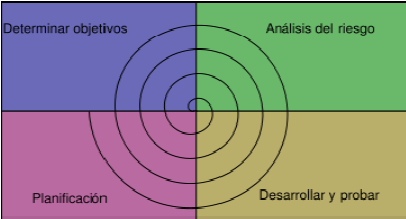
\includegraphics[width=1\linewidth]{1}
 	\caption{}
 	\label{fig:1}
 \end{figure}
 \\ \textbf{Planificar }
\\ • Se revisa el proyecto y se planifica la siguiente fase de la espiral.
 \\• Revisamos todo lo hecho, evaluándolo, y con ello decidimos si continuamos con las fases siguientes y planificamos la próxima
 actividad.\\ 
 
\vspace{8cm}
\textbf{Ventajas}
\\•La organizacion y actividades de las fases se encuentran bien definidas.
\\•Funciona bien para proyectos donde se encuentran bien definidos los requerimientos y el software que se desea.
\\•La planificacion es sencilla pues existe una secuencia bien 
definida de los pasos del proceso de software.
\\•La calidad del producto final es alta.\\ \\
\textbf{Desventajas}
\\•Lleva demasiado tiempo atravesar por todo el ciclo.
\\•Algunas fases pueden quedar pendientes.
\\•Cada giro se puede visualizar como una nueva version del 
sistema.\vspace{4cm}




\huge \textbf {Referencias} \\ \\ 
 \large\url{-http://computacion.cs.cinvestav.mx/~sperez/cursos/fis/Modelos.pdf}\\
\url{-http://www.ptolomeo.unam.mx:8080/xmlui/bitstream/handle/132.248.52.100/175/A5%20Cap%C3%ADtulo%202.pdf?sequence=5}\\


\end{document}